\documentclass[preprint,12pt]{elsarticle}

\usepackage[T1]{fontenc}
\usepackage{lmodern}
\usepackage{amsmath,amssymb}
\usepackage{graphicx}
\usepackage{booktabs}
\usepackage{url}
\usepackage[hidelinks]{hyperref}
\usepackage{microtype}
\usepackage{lineno}
\usepackage{array}

\journal{Biomedical Signal Processing and Control}
\graphicspath{{figures/}}

\begin{document}

\begin{frontmatter}

\title{Prescribed Force Trajectories as Benchmarks for Longitudinal EMG Decoding}

\author[ufpa]{Antonio Pereira\corref{cor1}}
\ead{apereira@ufpa.br}
\cortext[cor1]{Corresponding author.}
\affiliation[ufpa]{organization={Institute of Technology, Federal University of Par\'a},
  city={Bel\'em},
  state={Par\'a},
  postcode={66075--110},
  country={Brazil}}

\begin{abstract}
Longitudinal surface electromyography (sEMG) decoders are often evaluated in prescribed-force tasks, in which participants follow a predefined force trajectory. We quantified how much cross-day force-estimation accuracy could be obtained from task structure alone. Ten participants from the CEMHSEY GRASP dataset performed the same 30\% MVC cylindrical-grasp task over 11 consecutive days. Day 1 provided supervised calibration; on Days 2--11, Trial 1 supplied force-label-free session alignment and Trial 2 was held out. A protocol-defined temporal prior based solely on the prescribed 30-s trapezoidal target, with no parameters fitted from participant data, was compared with Day-1 force templates and 8- and 16-electrode state-space EMG decoders. Using physical sensor time bases, the prior achieved median participant-level $R^2=0.9933$, versus 0.9832 for the average Day-1 template and 0.9388 and 0.9370 for adaptive EMG decoding with eight and 16 electrodes. It exceeded the Day-1 average in 9/10 participants and all fixed and adaptive EMG decoders in all ten. After removal of repeatable residual structure, adaptive EMG residuals were positively correlated with force residuals in 88/100 and 89/100 evaluations, but residual $R^2$ was positive in only 0/100 and 1/100. The prior's advantage persisted under normalized-duration mapping. Session alignment and temporal filtering improved EMG-only decoding, whereas adaptive observation variance contributed little. Highly structured force protocols can themselves supply most of the apparent longitudinal predictability, while residual EMG information may remain associated with force without providing calibrated incremental prediction.
\end{abstract}

\begin{keyword}
surface electromyography \sep
force estimation \sep
longitudinal decoding \sep
temporal prior \sep
benchmarking \sep
high-density EMG
\end{keyword}

\end{frontmatter}

\linenumbers

\section{Introduction}

Surface electromyography (sEMG) provides non-invasive access to muscle activation and is widely used for proportional control in prosthetic, robotic, and rehabilitation interfaces \cite{Jiang2023,Farina2025}. A persistent challenge, however, is that the signal recorded at the skin can change across sessions because of differences in electrode placement, electrode--skin impedance, muscle state, fatigue, and other physiological or experimental factors. These changes alter the input seen by the decoder and can reduce performance after the initial calibration \cite{Wang2024}. Maintaining decoding performance across days is a central problem in longitudinal myoelectric control.

Most approaches to this problem seek to stabilize either the biosignal representation or the decoder. Random channel masking, for example, can reduce cross-day dependence on individual sEMG channels \cite{Jiang2022}, while domain-adaptation methods have been applied across sessions, participants, and fatigue states \cite{Li2024,Pan2025}. Adaptive decomposition can support online force prediction from motor-unit activity \cite{Zhao2024}, and recent motor-unit studies have examined cross-session force decoding and reliability \cite{Ruan2025,Roy2026,MengHu2026}. State-space models provide another strategy by exploiting the temporal continuity of force and reducing the influence of noisy observations \cite{Dutra2021,Dutra2023,Zhao2025StateSpace}. These methods address instability in the physiological signal and its mapping to force. More broadly, recent consensus guidance emphasizes that the validity of EMG-based force estimation depends strongly on the contraction, measurement, and biomechanical context \cite{Dick2024CEDE}. Longitudinal performance, however, can also depend on structure built into the task used to evaluate the decoder.

This second source of predictability becomes particularly important in prescribed-force tasks, in which participants attempt to follow a predefined force trajectory. If participants repeatedly increase force, hold it, and release it at prescribed times and amplitudes, elapsed task time alone carries information about the expected response. The prescribed schedule defines a protocol-defined temporal prior: an expected force trajectory that is available before observing either EMG or participant-specific force measurements. Under these conditions, a high cross-session $R^2$ can reflect both information carried by the biosignal and predictability imposed by the task. This distinction is especially relevant to the CEMHSEY GRASP protocol, in which participants followed the same 30\% MVC ramp--hold--release schedule across 11 consecutive days \cite{Yang2025}. Participant-specific force templates can also exploit this temporal regularity, but they require previously measured force from the participant. By contrast, the protocol-defined temporal prior is determined entirely by the experimental schedule.

The repeated CEMHSEY design provides an opportunity to separate predictability supplied by the task from information contributed by EMG. To determine whether high longitudinal decoding performance in this benchmark primarily reflects the prescribed temporal structure, physiological information carried by EMG, or both, we addressed three questions. First, how accurately does a protocol-defined temporal prior with no parameters fitted from participant data predict later-day force compared with participant-specific Day-1 templates and longitudinal EMG decoders? Second, after removing the participant-specific Day-1 force template and a repeatable residual trajectory, does EMG retain information about day-specific force deviations, and is that information calibrated well enough to improve prediction? Third, which components of the EMG-only decoder account for its cross-day performance? The primary analysis preserved the physical sampling rates of force and sEMG and used their common recording origin, while normalized-duration mapping was examined as a sensitivity analysis of temporal alignment. Together, these analyses establish how much longitudinal predictability is available from the experimental schedule alone and then quantify what the biosignal contributes beyond that benchmark.

\section{Materials and Methods}

\subsection{Dataset and longitudinal protocol}

We analyzed all ten GRASP participants contained in the CEMHSEY Part-I record (Subjects 1--10); the complete GRASP dataset contains 13 participants, with Subjects 11--13 distributed in Part II \cite{Yang2025}. The independent biological sample was $N=10$. For each participant we used Session 1, the cylindrical grasp, and Task 2 on 11 consecutive recording days. HD-sEMG was recorded from 320 channels at 2048~Hz and force at 200~Hz. According to the dataset documentation, the HD-sEMG acquisition used a gain of 150 and first-order high-pass and low-pass settings of 10~Hz and 4.4~kHz, respectively \cite{Yang2025}. The present reconstruction computed features directly from the provided \texttt{data\_sEMG} arrays; no additional software filtering or rectification was applied before feature extraction. The provided \texttt{data\_force} signal is dimensionless MVC-normalized force; no additional division by MVC was applied.

Task 2 prescribed 30\% MVC using a displayed trapezoidal target with real-time force feedback \cite{Yang2025}. The nominal schedule was 5~s at rest, a 5-s linear ramp from 0 to 0.30 MVC, a 10-s hold at 0.30 MVC, a 5-s linear ramp back to zero, and a final 5~s rest. This fixed schedule is central to the temporal-prior analysis below.

Day-1 Trial 1 was used for electrode ranking, feature standardization, regression fitting, and process-noise estimation. Day-1 Trial 2 was used for ridge and Kalman hyperparameter selection, baseline observation-noise estimation, the reference prediction distribution, and calibration of the hybrid model described below. On Days 2--11, Trial 1 supplied only EMG-derived predictions for session alignment; its force was not used by the decoder. Trial 2 was held out for scoring. The evaluation set contained 100 later-day participant-day recordings: ten evaluation days (Days 2--11) nested within each of ten participants. These repeated recordings increased within-participant longitudinal sampling but did not increase the independent biological sample beyond $N=10$.

The source study was approved by the academic ethics committee of Shanghai Jiao Tong University (E20240248I) and conducted in accordance with the Declaration of Helsinki. All participants provided informed consent \cite{Yang2025}.

\subsection{Feature extraction and force timing}

Mean absolute value (MAV), root mean square (RMS), and waveform length (WL) were computed independently for each electrode using 200-ms windows advanced by 100~ms. For samples $x_1,\ldots,x_N$ in a window, MAV was $N^{-1}\sum_n |x_n|$, RMS was $\sqrt{N^{-1}\sum_n x_n^2}$, and WL was $\sum_{n=2}^{N}|x_n-x_{n-1}|$. With the 2048-Hz sEMG stream this yielded 410-sample windows, a 205-sample step, and 299 feature windows per trial.

The primary force target used the physical sensor time bases. Force sample $n$ was assigned time $n/200$~s, and an EMG feature window was assigned the time of its center sample at 2048~Hz. Both streams used a common $t=0$; no lag was estimated or optimized. Force was linearly interpolated to the EMG-window centers. As a sensitivity analysis, the complete comparison was repeated after mapping force and EMG to normalized trial duration. No held-out force label was used to choose the synchronization convention.

\subsection{EMG-only decoder}

Electrodes were ranked by the absolute Pearson correlation between Day-1 Trial-1 MAV and force. The highest-ranked $k\in\{8,16\}$ electrodes were retained. For each selected electrode, MAV, RMS, and WL were standardized using Day-1 Trial-1 means and population standard deviations and entered into an independent ridge regression. The penalty was selected independently for each electrode from 17 logarithmically spaced values between $10^{-3}$ and $10^5$ using Day-1 Trial-2 mean-squared error.

The independent electrode predictions $z_{i,t}$ were combined in two stages. First, later-day Trial 1 supplied a force-label-free session alignment. Let the robust consensus prediction on Day-1 Trial 2 have median $c_{\mathrm{ref}}$ and interquartile range $s_{\mathrm{ref}}$, and let the later-day Trial-1 consensus have corresponding values $c_d$ and $s_d$. Test-trial electrode predictions were transformed as
\begin{equation}
\tilde z_{i,t}=c_{\mathrm{ref}}+\frac{s_{\mathrm{ref}}}{s_d}\left(z_{i,t}-c_d\right).
\end{equation}
The consensus at each time point was the arithmetic mean after excluding observations farther than three scaled median absolute deviations from the cross-electrode median.

Second, the aligned predictions entered a scalar random-walk Kalman filter,
\begin{align}
x_t &= x_{t-1}+w_t, & w_t&\sim\mathcal N(0,Q),\\
\tilde z_{i,t} &= x_t+v_{i,t}, & v_{i,t}&\sim\mathcal N(0,R_{i,t}).
\end{align}
For electrode $i$, baseline observation variance was the Day-1 Trial-2 residual mean square,
\begin{equation}
R_{i,0}=\frac{1}{T}\sum_{t=1}^{T}\left(y_t-z_{i,t}\right)^2,
\end{equation}
where $T$ is the number of Day-1 Trial-2 feature windows. In the fixed-variance model, $R_{i,t}=R_{i,0}$. In the adaptive model, let $m_t=\operatorname{median}(z_{1,t},\ldots,z_{k,t})$ and let $s_t=1.4826\,\mathrm{MAD}(z_{1,t},\ldots,z_{k,t})$. Robust cross-electrode disagreement was
\begin{equation}
d_{i,t}=\frac{|z_{i,t}-m_t|}{s_t+\epsilon},
\end{equation}
where $\epsilon>0$ is a numerical safeguard against division by zero. The adaptive observation variance was
\begin{equation}
R_{i,t}=R_{i,0}\exp\!\left[\min(\alpha d_{i,t}^2,12)\right].
\end{equation}
The process variance was $Q=q_s\operatorname{Var}(\Delta y)$ from Day-1 Trial 1. Values $q_s\in\{0.01,0.03,0.1,0.3,1,3,10\}$ and $\alpha\in\{0,0.1,0.25,0.5,1,2\}$ were selected using Day-1 Trial-2 error and then fixed for all later recordings.

\subsection{Temporal-prior benchmarks}

The primary temporal benchmark was the nominal Task-2 protocol target, which used no force measurement and had no fitted amplitude, offset, time shift, or lag. At elapsed time $t$ in seconds,
\begin{equation}
T_{\mathrm{nom}}(t)=
\begin{cases}
0, & 0\le t<5,\\
0.30(t-5)/5, & 5\le t<10,\\
0.30, & 10\le t<20,\\
0.30(25-t)/5, & 20\le t<25,\\
0, & 25\le t\le 30.
\end{cases}
\end{equation}
The target was evaluated directly at the same physical EMG-window center times used for scoring.

Two participant-specific time-only benchmarks were also retained. One used the Day-1 Trial-1 measured force trajectory as a function of elapsed task time. The second averaged the two Day-1 measured force trajectories. For each later held-out recording these templates were evaluated at the same feature-window times. The empirical templates used initial-day force measurements; $T_{\mathrm{nom}}$ represented the protocol schedule alone.

\subsection{Calibration-only hybrid}

To examine whether an EMG contribution calibrated on Day 1 transferred to later recordings, a one-parameter hybrid was fitted separately for each participant and electrode count. Let $T_1(t)$ be the Day-1 Trial-1 temporal template and $E(t)$ the EMG decoder prediction. On Day-1 Trial 2 we fitted
\begin{equation}
\hat y(t)=T_1(t)+\beta\,[E(t)-T_1(t)],
\end{equation}
with $\beta$ constrained to $[0,1]$. The fitted $\beta$ was then frozen for all Days 2--11. Because Day-1 Trial 2 was used to estimate $\beta$, fit quality on that recording describes calibration performance and does not provide independent validation evidence. Later-day Trial-2 recordings were used to assess transfer. The hybrid was compared with the single-trial template used in its equation and with the average template formed from both Day-1-trials.

\subsection{Secondary component analysis of the EMG branch}

A secondary reconstruction isolated the contributions of session alignment, temporal filtering, and disagreement-driven variance adaptation. Alignment compared aligned and unaligned robust consensus predictions. Temporal filtering compared a fixed-variance Kalman filter with instantaneous inverse-variance-weighted fusion using the same observation variances. Fast adaptation compared the adaptive Kalman filter with an $\alpha=0$ filter at the same selected process-noise scale. This component analysis used the normalized-duration target; the separate timing sensitivity tested whether the main conclusions depended on that convention.

\subsection{Performance and inference}

For each held-out Trial 2 we computed
\begin{equation}
R^2=1-\frac{\sum_t(y_t-\hat y_t)^2}{\sum_t(y_t-\bar y)^2},
\end{equation}
RMSE, RMSE normalized by the target standard deviation, MAE, signed bias, and prediction--target correlation. Each participant contributed the median across ten later-day recordings, and cohort summaries used the median across the ten participants. Participant-wise paired effects were summarized by the median paired difference with a 95\% percentile bootstrap interval from 100,000 resamples of the $N=10$ participants with replacement. The participant was the inferential unit for these comparisons; recordings and feature windows were treated as repeated observations within participants. Two-sided Wilcoxon signed-rank tests were used as exploratory participant-level paired tests. For the five primary nominal-target contrasts (nominal target versus the average Day-1 template and versus fixed/adaptive EMG at two electrode counts), Holm adjustment controlled the comparison family. The secondary three-stage EMG component family used Holm adjustment across six $R^2$ tests formed by three stages and two electrode counts. Hybrid contrasts are reported descriptively with unadjusted exploratory signed-rank tests. Because the temporal-prior benchmark was introduced after reconstruction exposed strong task stereotypy, all inferential comparisons are exploratory and were not preregistered as confirmatory tests.

Residual analyses were descriptive. First, observed force and EMG prediction were residualized against the average Day-1 measured-force template. To test whether the resulting correlation merely reflected a repeatable residual waveform, each later day was then treated in turn as held out. For that day, the mean true-residual trajectory and mean prediction-residual trajectory were computed from the other nine evaluation days of the same participant and subtracted from the held-out residuals. Pearson correlation and residual $R^2$ were then calculated between these leave-one-day-out residual series. This nuisance-removal control uses force labels from other evaluation days, so it cannot serve as a deployable prediction procedure. Its purpose is to diagnose residual association after removal of repeatable time-locked structure. The resulting 100 participant-day evaluations comprise ten repeated days nested within each of ten participants and are summarized descriptively; they are not treated as 100 independent inferential observations. No individual-window significance test is used for confirmatory inference because the trajectories are temporally autocorrelated.

ChatGPT (\mbox{OpenAI}) was used to assist with analysis-code development and interpretation of diagnostic outputs during the reconstruction. The reported numerical analyses were performed using conventional data-processing and statistical code. The author reviewed the analytical choices and assumes responsibility for the results.

\section{Results}

\subsection{Protocol-Defined Temporal Prior}

The prescribed target, which used no parameters fitted from participant data, was the strongest longitudinal predictor. Using the physical sensor time bases, the nominal 30\%-MVC trapezoid reached a cohort median participant-level $R^2$ of 0.9933, median RMSE of 0.0106, and a participant-median $R^2$ range of 0.9853--0.9958. The average of the two measured Day-1 force trajectories reached $R^2=0.9832$, while the single Day-1 Trial-1 template reached 0.9801. Fixed-variance EMG decoding reached 0.9335 with eight electrodes and 0.9356 with 16; adaptive decoding reached 0.9388 and 0.9370, respectively (Table~\ref{tab:main}; Fig.~\ref{fig:main}).

Relative to the Day-1 average force template, the nominal protocol prior improved participant median $R^2$ by 0.00866 (95\% bootstrap CI 0.00318--0.02729) and was better in 9/10 participants and 80/100 held-out recordings. It exceeded fixed and adaptive EMG decoding in all ten participant summaries at both electrode counts and in 99--100 of 100 held-out recordings. Across the five nominal-target contrasts, Holm-adjusted signed-rank $p=0.0098$ for each comparison (Table~\ref{tab:nominal}).

\begin{figure}[t]
\centering
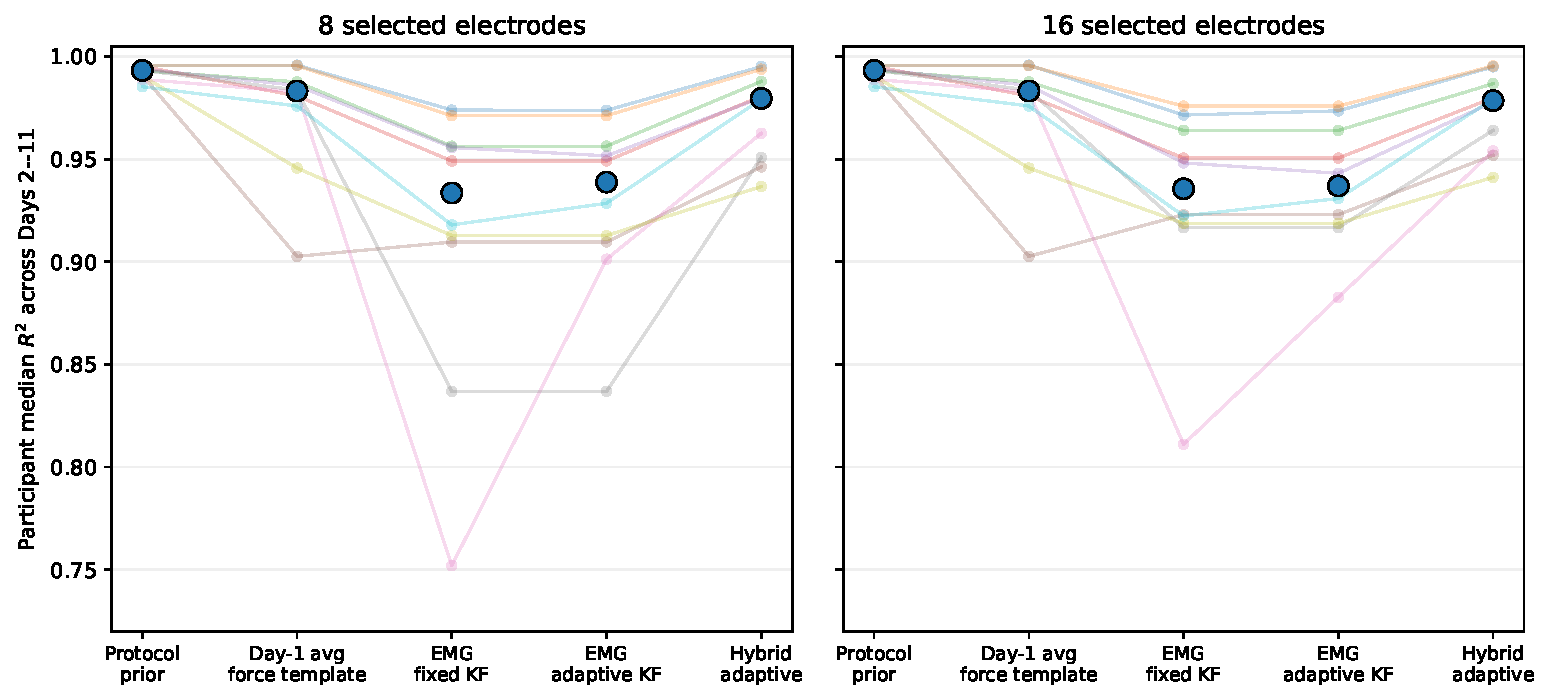
\includegraphics[width=\linewidth]{fig1_temporal_prior_vs_emg.pdf}
\caption{Participant-level longitudinal performance using the physical sensor time bases. Thin lines connect methods within each participant; large symbols show cohort medians. The protocol prior is the nominal 30\%-MVC trapezoid with no parameters fitted from participant data and uses no measured force or EMG. The Day-1 average template uses the two initial-day measured force trajectories. EMG models use later-day EMG but no later-day force for fitting or adaptation; the adaptive hybrid uses a Day-1-fitted scalar EMG weight.}
\label{fig:main}
\end{figure}

\begin{table}[t]
\caption{Longitudinal performance using the physical sensor time bases}
\label{tab:main}
\centering
\small
\begin{tabular}{lcccc}
\toprule
& \multicolumn{2}{c}{8 electrodes} & \multicolumn{2}{c}{16 electrodes}\\
\cmidrule(lr){2-3}\cmidrule(lr){4-5}
Method & Median $R^2$ & RMSE & Median $R^2$ & RMSE\\
\midrule
Nominal protocol prior & \textbf{0.9933} & \textbf{0.0106} & \textbf{0.9933} & \textbf{0.0106}\\
Day-1 Trial-1 template & 0.9801 & 0.0180 & 0.9801 & 0.0180\\
Day-1 average template & 0.9832 & 0.0170 & 0.9832 & 0.0170\\
EMG fixed KF & 0.9335 & 0.0325 & 0.9356 & 0.0318\\
EMG adaptive KF & 0.9388 & 0.0313 & 0.9370 & 0.0317\\
Hybrid adaptive & 0.9796 & 0.0182 & 0.9785 & 0.0187\\
\bottomrule
\end{tabular}
\end{table}

\begin{table}[t]
\caption{Exploratory participant-wise contrasts for the nominal protocol prior}
\label{tab:nominal}
\centering
\small
\setlength{\tabcolsep}{4pt}
\begin{tabular}{lrrrr}
\toprule
Comparator & Median $\Delta R^2$ & 95\% CI & Improved & Holm $p$\\
\midrule
Day-1 average template & 0.00866 & $[0.00318,0.02729]$ & 9/10 & 0.0098\\
Fixed EMG, 8 & 0.05674 & $[0.03143,0.11712]$ & 10/10 & 0.0098\\
Adaptive EMG, 8 & 0.05145 & $[0.03347,0.08268]$ & 10/10 & 0.0098\\
Fixed EMG, 16 & 0.05434 & $[0.02915,0.07233]$ & 10/10 & 0.0098\\
Adaptive EMG, 16 & 0.05262 & $[0.02915,0.07233]$ & 10/10 & 0.0098\\
\bottomrule
\end{tabular}
\end{table}

\subsection{EMG Beyond the Temporal Prior}

The Day-1 hybrid fit assigned nonzero weight to EMG for most participants: median fitted $\beta$ was 0.367 with eight electrodes and 0.338 with 16 (Fig.~\ref{fig:incremental}A). These values describe the calibration fit and are not independent validation results because $\beta$ was estimated on Day-1 Trial 2. On later held-out days, the adaptive hybrid did not improve consistently on the stronger average Day-1 force template. Median paired $\Delta R^2$ was $-0.00119$ (95\% CI $-0.0131$ to 0.00161, exploratory signed-rank $p=0.322$) with eight electrodes and $-0.00089$ (95\% CI $-0.0121$ to 0.00127, $p=0.232$) with 16; only 3/10 and 2/10 participant summaries improved, respectively (Fig.~\ref{fig:incremental}B). The adaptive-hybrid cohort medians of 0.9796 and 0.9785 also remained below the nominal protocol prior.

\begin{figure}[t]
\centering
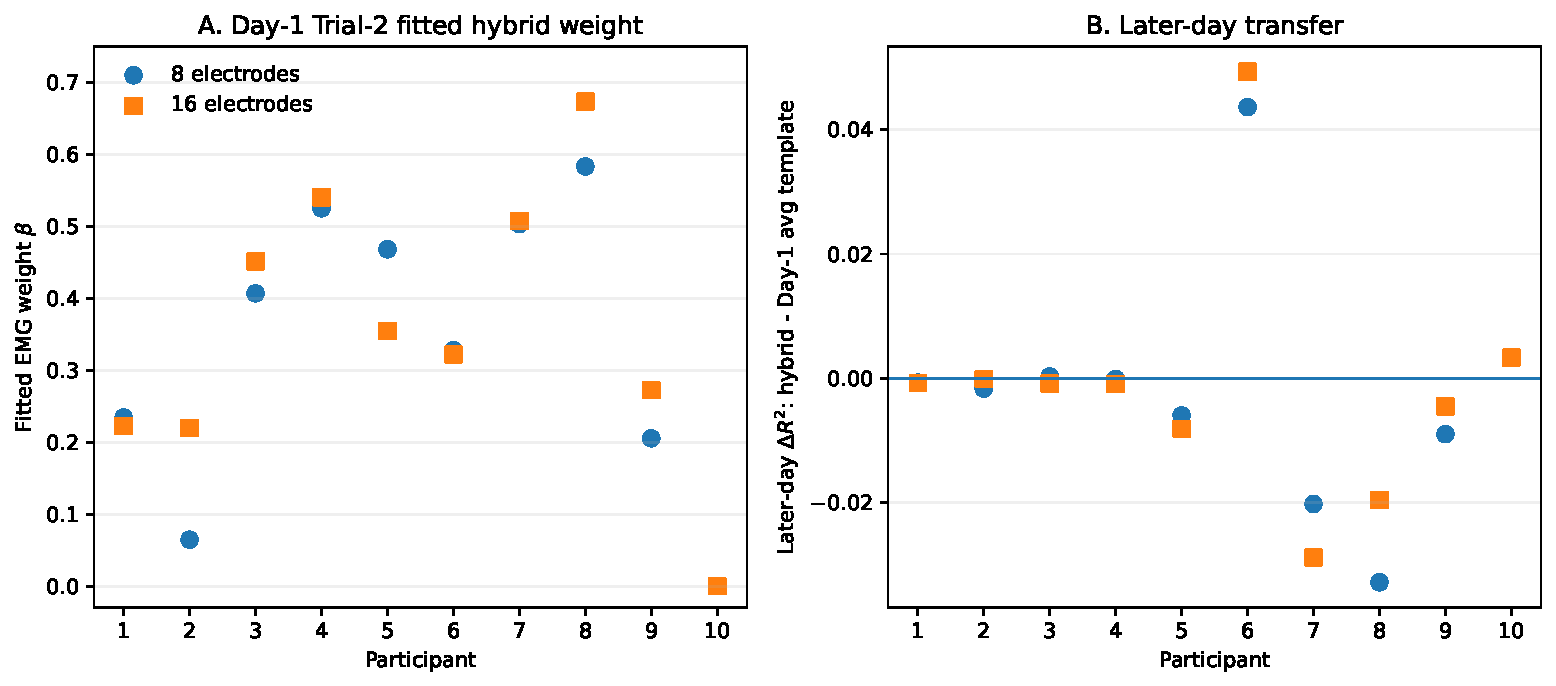
\includegraphics[width=\linewidth]{fig2_incremental_emg.pdf}
\caption{Day-1-fitted hybrid and later-day transfer. (A) Fitted EMG weight $\beta$ on Day-1 Trial 2; these values are calibration parameters, not independent validation evidence. (B) Participant-level later-day difference between the adaptive hybrid and the average Day-1 measured-force template. Subject 6 was the clearest positive exception, but most differences were near zero or negative.}
\label{fig:incremental}
\end{figure}

The stricter residual-shape control supported residual association but not calibrated residual-force prediction. Across the 100 held-out participant-day evaluations (ten days nested within each of ten participants), after subtracting the Day-1 average template and then removing, for each held-out day, the mean residual shape estimated from the other nine evaluation days of the same participant, adaptive EMG residuals were positively correlated with force residuals in 88/100 evaluations with eight electrodes and 89/100 with 16. Median recording-level correlations were 0.357 and 0.355, respectively. However, residual $R^2$ was positive in only 0/100 and 1/100 evaluations, with median residual $R^2=-5.31$ and $-4.10$. Fixed-variance EMG produced the same qualitative pattern: correlations were positive in 87/100 and 89/100 evaluations, whereas residual $R^2$ was positive in 0/100 and 1/100. These counts are descriptive frequencies of repeated participant-day evaluations, not an $N=100$ inferential sample. Because the nuisance trajectory uses force labels from other evaluation days, this analysis is descriptive and cannot be deployed for prediction. Positive residual association persisted after removal of repeatable temporal structure, but residual amplitude was generally not calibrated sufficiently to yield positive out-of-sample $R^2$.

\begin{figure}[t]
\centering
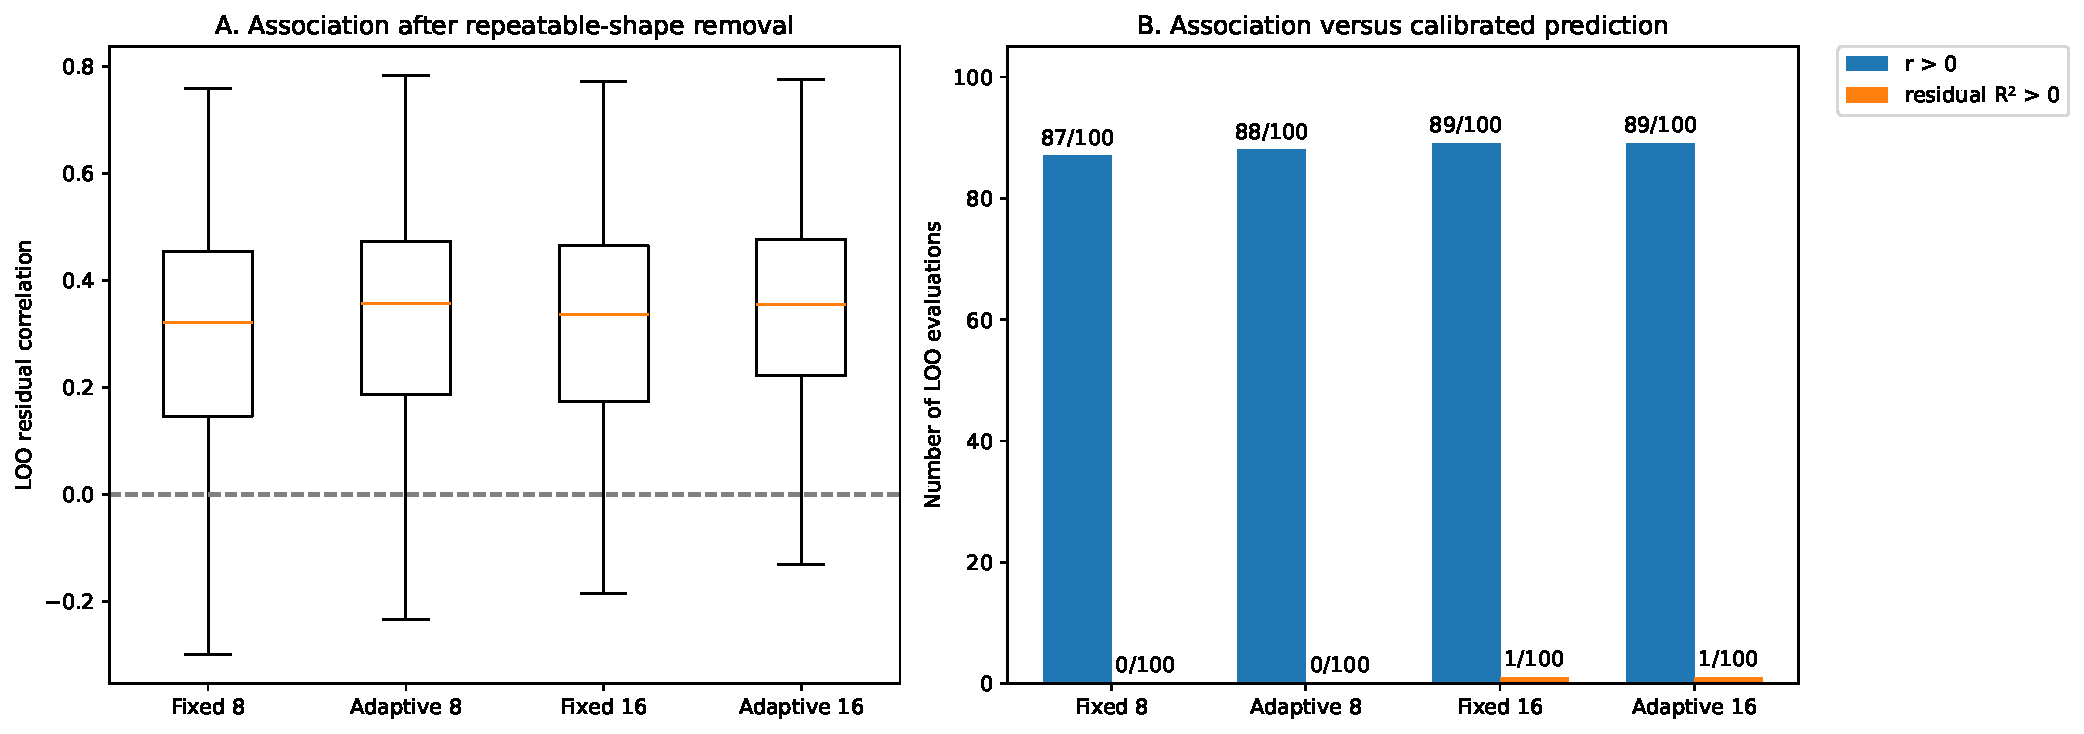
\includegraphics[width=\linewidth]{fig3_residual_information_final.pdf}
\caption{Leave-one-day-out residual-shape diagnostic using the physical time base. Each configuration contains 100 participant-day evaluations: ten held-out days (Days 2--11) nested within each of ten participants. For each held-out day, the average true-residual and prediction-residual trajectories from the other nine evaluation days of the same participant were removed before comparison. (A) Distribution of residual correlations across the 100 descriptive evaluations. (B) Number of evaluations with positive correlation and with positive residual $R^2$. These repeated evaluations do not represent 100 independent participants and are not used as an $N=100$ inferential sample. The diagnostic uses force labels from other evaluation days to remove nuisance structure and cannot be deployed for prediction.}
\label{fig:residual}
\end{figure}

\subsection{Time-Base Sensitivity}

The temporal-prior result was stable to the choice of time mapping. The nominal target reached a cohort median participant-level $R^2=0.99327$ using the physical force time base and 0.99207 after normalized-duration mapping. Its median paired advantage over the Day-1 average template was 0.00866 and 0.00792 under the two mappings, respectively. The Day-1 average template was similarly stable ($R^2=0.98323$ versus 0.98355), and EMG-only and hybrid methods showed no consistent change. The close agreement across the two analyses indicates that normalized-duration warping was not responsible for the observed temporal-prior advantage.

\subsection{EMG-Only Adaptation}

The EMG-only decoder still benefited from session alignment and temporal filtering. In the secondary component analysis, session alignment increased participant-level $R^2$ by a median 0.0817 with eight electrodes and 0.0689 with 16; 9/10 participants improved in both configurations, with Holm-adjusted $p=0.039$ (Fig.~\ref{fig:ablation}). With the same fixed observation weights, Kalman temporal filtering added median paired gains of 0.00963 and 0.01166; all ten participants improved for both electrode counts (Holm-adjusted $p=0.0117$). In contrast, removing disagreement-driven adaptive variance while keeping the process-noise scale fixed produced median paired $\Delta R^2=0$ for both electrode counts; only four participants improved and six were unchanged in each configuration (Holm-adjusted $p=0.25$). Consistently, $\alpha=0$ was selected during Day-1 calibration in 12 of 20 participant/electrode-count fits.

The largest coherent scale failure occurred in Subject 6. Under the normalized-duration reconstruction, the eight-electrode robust consensus had median later-day $R^2=-2.440$ before alignment and 0.905 after alignment, corresponding to $\Delta R^2=+3.344$; with 16 electrodes the corresponding values were $-3.041$ and 0.910, giving $\Delta R^2=+3.951$. Values of $\Delta R^2$ greater than one are possible because $R^2$ is unbounded below. Direct verification against the saved prediction traces confirmed that these large gains arose from strongly negative unaligned baselines and were not plotting or arithmetic errors. This case illustrates why cross-electrode agreement alone cannot guarantee preservation of the force scale. The dominant longitudinal gain in the reconstructed EMG pipeline came from session-level alignment; fast variance adaptation contributed little.

\begin{figure}[t]
\centering
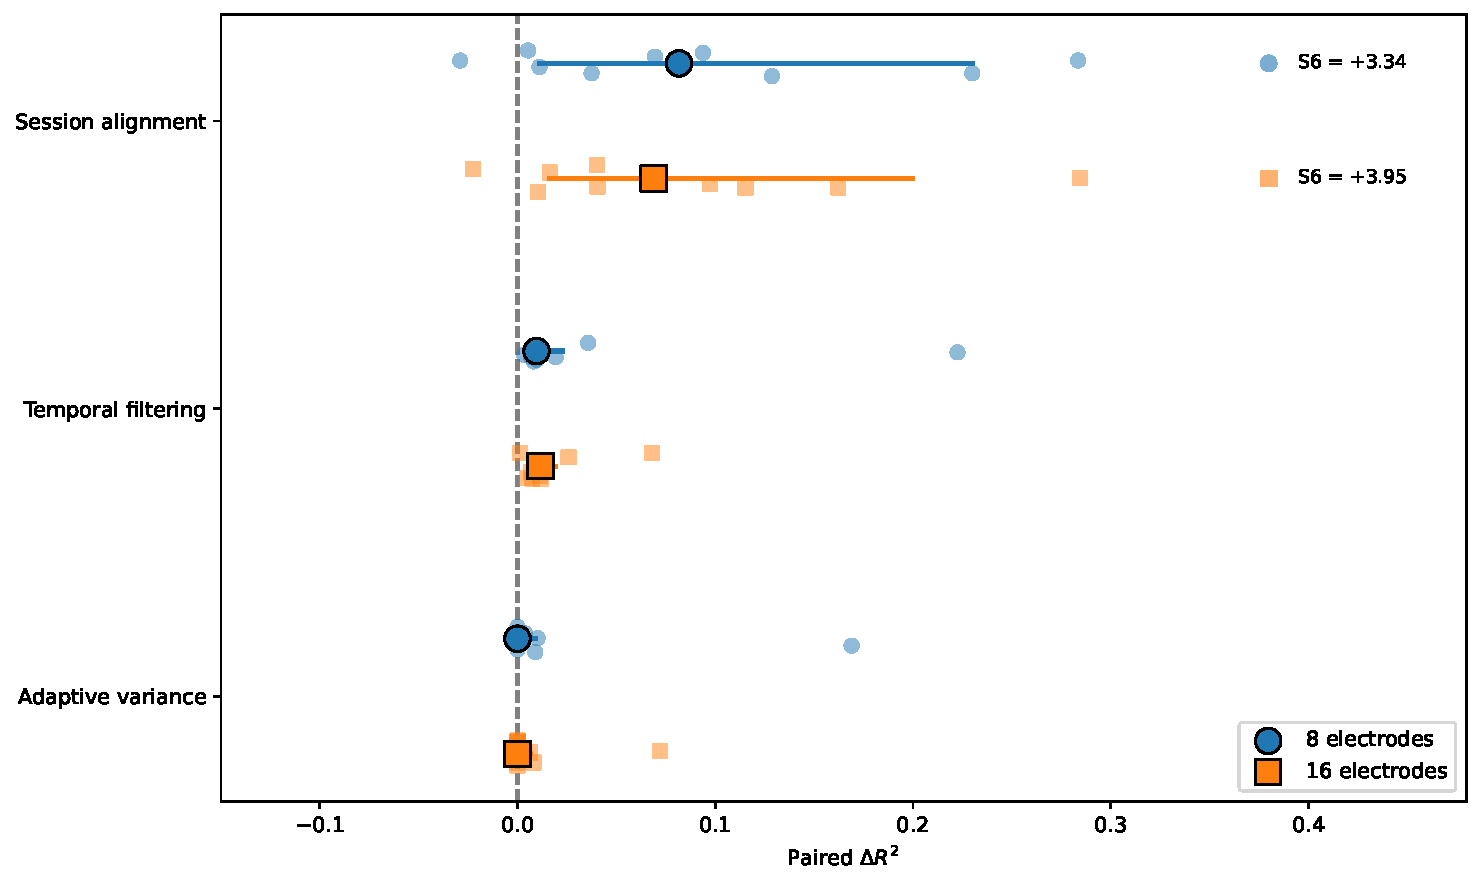
\includegraphics[width=0.92\linewidth]{fig4_emg_component_ablation_final.pdf}
\caption{Secondary component analysis of the EMG-only decoder using normalized-duration mapping. Small points show paired $\Delta R^2$ for each participant ($N=10$); large outlined symbols show the cohort median, and horizontal lines show 95\% percentile intervals from 100,000 participant-level bootstrap resamples. The Subject-6 session-alignment effects ($\Delta R^2=+3.34$ for eight electrodes and $+3.95$ for 16) are annotated off scale; values greater than one are possible because the corresponding unaligned baseline $R^2$ values were strongly negative. Session alignment produced the largest gain, temporal filtering produced a smaller positive gain, and adaptive observation variance showed little additional effect when compared at the same process-noise scale.}
\label{fig:ablation}
\end{figure}

\begin{table}[t]
\caption{Secondary EMG-only component effects on participant median $R^2$}
\label{tab:ablation}
\centering
\small
\begin{tabular}{llrrr}
\toprule
Component & $k$ & Median $\Delta R^2$ & 95\% CI & Holm $p$\\
\midrule
Session alignment & 8 & 0.0817 & $[0.0111,0.2301]$ & 0.039\\
Session alignment & 16 & 0.0689 & $[0.0164,0.2000]$ & 0.039\\
Temporal filtering & 8 & 0.00963 & $[0.00777,0.0227]$ & 0.0117\\
Temporal filtering & 16 & 0.01166 & $[0.00622,0.0194]$ & 0.0117\\
Adaptive variance & 8 & 0.0000 & $[0.0000,0.00899]$ & 0.250\\
Adaptive variance & 16 & 0.0000 & $[0.0000,0.00646]$ & 0.250\\
\bottomrule
\end{tabular}
\end{table}

\section{Discussion}

Longitudinal EMG force decoding is usually framed as a problem of preserving a stable physiological mapping across sessions. Accordingly, recent work has focused on stabilizing the biosignal representation or decoder through regularization, domain adaptation, state-space estimation, and motor-unit representations \cite{Jiang2022,Wang2024,Li2024,Pan2025,Dutra2021,Ruan2025,Roy2026,MengHu2026}. Our results identify an additional and more basic issue in prescribed-force benchmarks: a large fraction of apparent longitudinal predictability may already be supplied by the experimental protocol. A 30\%-MVC trapezoid defined only by the instructed ramp--hold--release schedule, with no parameters fitted from participant data, reached a median participant-level $R^2=0.9933$ across Days 2--11. It outperformed both the mean of two measured Day-1 force trajectories ($R^2=0.9832$) and the EMG-only state-space decoders ($R^2<0.94$). Thus, the strongest longitudinal predictor in this benchmark contained neither EMG nor participant-specific force measurements.

The implication of this finding is that high cross-session accuracy in a stereotyped task does not necessarily indicate that a decoder has overcome physiological nonstationarity. When task instructions and elapsed time already specify a highly repeatable force trajectory, prediction accuracy combines information carried by the biosignal with information imposed by the experimental design. In the present dataset, the nominal protocol prior required no measured force, EMG, fitted amplitude, offset, timing shift, or lag, yet it still outperformed the physiological decoders. A protocol-defined temporal prior provides a direct control for determining how much of the apparent longitudinal performance is attributable to the biosignal itself.

EMG nevertheless retained information about day-specific departures from the repeated force trajectory. After removing the Day-1 temporal template and an additional repeatable residual trajectory estimated from the other nine evaluation days, EMG residual predictions remained positively correlated with force residuals in most recordings. For adaptive decoding, the median residual correlation was approximately 0.36 at both electrode counts. Correlation alone, however, did not translate into accurate prediction of residual-force magnitude. Residual $R^2$ was positive in none of the 100 participant-day evaluations with eight electrodes and in only one of 100 evaluations with 16 electrodes. The EMG residuals tracked some day-specific variation in force, but their amplitude was generally not calibrated well enough to reconstruct that variation accurately. The leave-one-day-out nuisance removal is not a deployable procedure because it uses force labels from other evaluation days; its role here is diagnostic. It shows that the residual EMG--force association cannot be explained solely by a repeatable residual waveform shared across days.

The hybrid analysis reached a similar conclusion from a different direction. Fitting the hybrid model on Day-1 Trial 2 produced nonzero EMG weights for most participants, showing that EMG could explain force variation beyond the temporal template within that calibration recording. Those weights, however, were estimated from the same recording and do not provide independent evidence of generalization. Once the fitted weights were frozen and applied to later days, the hybrid model did not consistently outperform the stronger Day-1 average template and remained below the nominal protocol prior at the cohort level. EMG thus provided an incremental relationship with force during calibration, but that relationship did not transfer across days with sufficiently stable amplitude calibration to improve the temporal benchmark consistently.

The timing analysis further showed that this result was not created by normalized-duration warping. The protocol prior remained near $R^2=0.99$ under both physical-time and normalized-duration mappings, and its advantage over the Day-1 average template remained positive. No lag was optimized on held-out recordings. The persistence of the result under both mappings links the strong temporal prediction to the repeated prescribed trajectory, not to either synchronization convention. Other preprocessing or alignment choices could still affect individual estimates, but they are unlikely to account for the central result.

The EMG-only analysis remains informative because it identifies which components of the physiological decoder improved cross-session robustness. Session alignment produced the largest gain within the reconstructed EMG branch, while temporal state-space filtering provided a smaller but consistent additional improvement. These results are consistent with the sensitivity of sEMG to cross-session distribution shifts \cite{Wang2024,Li2024} and with the value of temporal state-space structure for continuous myoelectric estimation \cite{Dutra2021,Dutra2023,Zhao2025StateSpace}. By contrast, disagreement-driven variance adaptation contributed little. Removing it while keeping the same process-noise scale produced essentially no change in median performance, and calibration selected $\alpha=0$ in 12 of 20 participant/configuration fits. The longitudinal gains observed in this dataset were driven mainly by session-level alignment and temporal filtering; rapid electrode-specific reweighting contributed little.

Subject 6 illustrates why protocol predictability and physiological decoding should be considered separately. Its unaligned electrode predictions showed a large coherent scale shift across sessions that was substantially corrected by force-label-free session alignment. It was also the clearest participant for whom the later-day hybrid model exceeded the Day-1 average force template. EMG can provide useful participant-specific information beyond the repeated task trajectory. Across the cohort, however, that contribution was less stable across participants and sessions than the temporal structure imposed by the protocol. Experimental designs with randomized target timing, randomized force amplitudes, self-paced contractions, or perturbations that decorrelate force from elapsed time would place greater demands on the physiological signal and provide a more stringent test of longitudinal EMG decoding.

Several limitations define the scope of these conclusions. The independent biological sample comprised $N=10$ participants (Subjects 1--10 from the CEMHSEY Part-I GRASP record), and the analysis was restricted to one cylindrical grasp at one prescribed force level. The ten evaluation days per participant provide dense longitudinal sampling within individuals, but they do not increase the independent biological sample size. The small biological sample limits population-level generalization and precise estimation of between-participant heterogeneity. The protocol prior also assumes knowledge of task onset and the prescribed target trajectory. It is intended as a benchmarking control for structured experiments, not as a decoder for unconstrained behavior.

Other limitations concern the roles assigned to calibration and evaluation recordings. Day-1 Trial 2 was used for several calibration steps, including hyperparameter selection and hybrid-weight fitting, and does not constitute an independent validation recording. Similarly, the leave-one-day-out residual-shape analysis uses force labels from other evaluation days and is explicitly descriptive; it cannot be used for deployment. The primary force/EMG timing analysis used a common $t=0$ without optimizing a lag, although normalized-duration mapping produced the same substantive result. Finally, the protocol-defined benchmark was introduced after reconstruction of the original decoding pipeline revealed strong trajectory stereotypy. The corresponding inferential comparisons should be considered exploratory. A prospective test should define the temporal baseline in advance and evaluate it in protocols that deliberately vary target timing, amplitude, or both. Such designs would make performance less predictable from elapsed time and provide a cleaner estimate of the information that longitudinal EMG decoding contributes beyond the experimental schedule.

\section{Conclusion}

The main finding of this study was that a protocol-defined temporal prior based on the prescribed 30\%-MVC target, with no parameters fitted from participant data, predicted held-out later-day force more accurately than participant-specific Day-1 templates or longitudinal EMG decoders. EMG predictions retained a positive association with day-specific force residuals after removal of repeatable temporal structure, but that association almost never yielded positive residual $R^2$. The residual EMG signal showed association without generally calibrated force prediction. Within the EMG-only branch, session alignment and temporal filtering improved longitudinal decoding, whereas disagreement-driven adaptive observation variance added little overall. Longitudinal biosignal studies using stereotyped prescribed tasks should include protocol-defined temporal priors as benchmarks before interpreting high cross-session accuracy as evidence of information extracted from the physiological signal.

\section*{Data and Code Availability}
The CEMHSEY Part-I GRASP dataset analyzed in this study is publicly available from Zenodo (DOI: 10.5281/zenodo.14224328) \cite{Yang2025}. The versioned reproducibility archive is available from Zenodo (v1.0.1, DOI: \mbox{10.5281/zenodo.23249424}) and the \href{https://github.com/squareshorts/emg-longitudinal-temporal-prior/releases/tag/v1.0.1}{GitHub v1.0.1 release}. The archive contains code implementing the protocol-defined temporal-prior and Day-1 force-template comparisons, fixed analysis specifications, and numerical summaries of the EMG, hybrid, residual, and component analyses. The complete execution pipeline and intermediate outputs for these secondary analyses are not included.

\section*{Competing Interests}
The author declares no competing interests.

\section*{Declaration of generative AI and AI-assisted technologies in the manuscript preparation process}
ChatGPT (\mbox{OpenAI}) assisted with technical writing and language revision during manuscript preparation. The author reviewed and edited the resulting text and takes full responsibility for the article.

\bibliographystyle{elsarticle-num}
\bibliography{references}

\end{document}
